\documentclass[11pt]{beamer}

\usetheme{metropolis}

\usepackage{graphicx}
\usepackage{physics}
\usepackage{adjustbox}
\usepackage{caption}
\usepackage{chemformula}
\usepackage{quoting}
\usepackage[style=chem-angew,backend=bibtex]{biblatex}
\bibliography{references}
%
% Choose how your presentation looks.
%
% For more themes, color themes and font themes, see:
% http://deic.uab.es/~iblanes/beamer_gallery/index_by_theme.html
%
\mode<presentation>
{
  \usetheme{default}      % or try Darmstadt, Madrid, Warsaw, ...
  \usecolortheme{default} % or try albatross, beaver, crane, ...
  \usefonttheme{default}  % or try serif, structurebold, ...
  \setbeamertemplate{navigation symbols}{}
  \setbeamertemplate{caption}[numbered]
  \setbeamerfont{footnote}{size=\tiny}
} 

\usepackage[english]{babel}
\usepackage[utf8]{inputenc}
\graphicspath{{image/}}

\AtBeginSection[]{
\begin{frame}{Outline}
  \tableofcontents[currentsection]
\end{frame}
}

\title{Chapter 3: Chemical Compounds}
\institute{Chemistry Department, Cypress College}
\date{Sept 7, 2022}

\begin{document}

\begin{frame}
  \titlepage
\end{frame}

\begin{frame}{Class Announcements}
  \begin{itemize}
  \item Inputted grades for up to the quiz
  \item When uploading assignments, be certain that
    the file is in a readable format e.g. docx, png, jpeg,
    and pdf
  \item Everyone performed pretty well on the quiz; average
    4.1 and standard deviation 0.84
  \item This week only, any late assignments will not be
    penalized $50\%$; submit late assignments by the Sept 7th
    at 11:59pm
  \item Quiz \#2 released this Thurs, Sept 8 at 11am and due Mon,
    Sept 12 at 11am
  \item Homework \#2 released this Fri, Sept 9 at 11am and due
    Fri, Sept 16 at 11am
  \end{itemize}  
\end{frame}

\begin{frame}{Lecture and Lab Weekly Agenda}
  \textbf{Lab Section}

  \begin{itemize}
  \item Finish Exp 1 - Laboratory Techniques
  \item There is no need to cut glassware and fire
    polishing
  \item Be familiarize with evaporation and filtration
    techniques
  \item Submit the lab worksheet due Sept 14 at 11:59pm;
    $50\%$ late penalty 
  \end{itemize}

  \textbf{Lecture Section}

  \begin{itemize}
  \item Go over homework assignment; present your work
    for 1pt EC
  \item Review Ch 2 - Atoms, Ions, and the Periodic Table
  \item Begin lecture on Ch 3 - Chemical Compounds and
    Ch 8.1 - 8.2 - Types of Bonding
  \end{itemize}
\end{frame}

\section{Review: Chapter 2 Highlights}

\begin{frame}{Atoms and Ions}
  \begin{itemize}
  \item Conservation of mass and conservation of energy
  \item Anions (gain electron) and cations (lose electron)
  \item Made up of protons, neutrons, and electrons
  \end{itemize}
\end{frame}

\begin{frame}{J.J. Thompson's Plum Pudding Model}
  \centering
  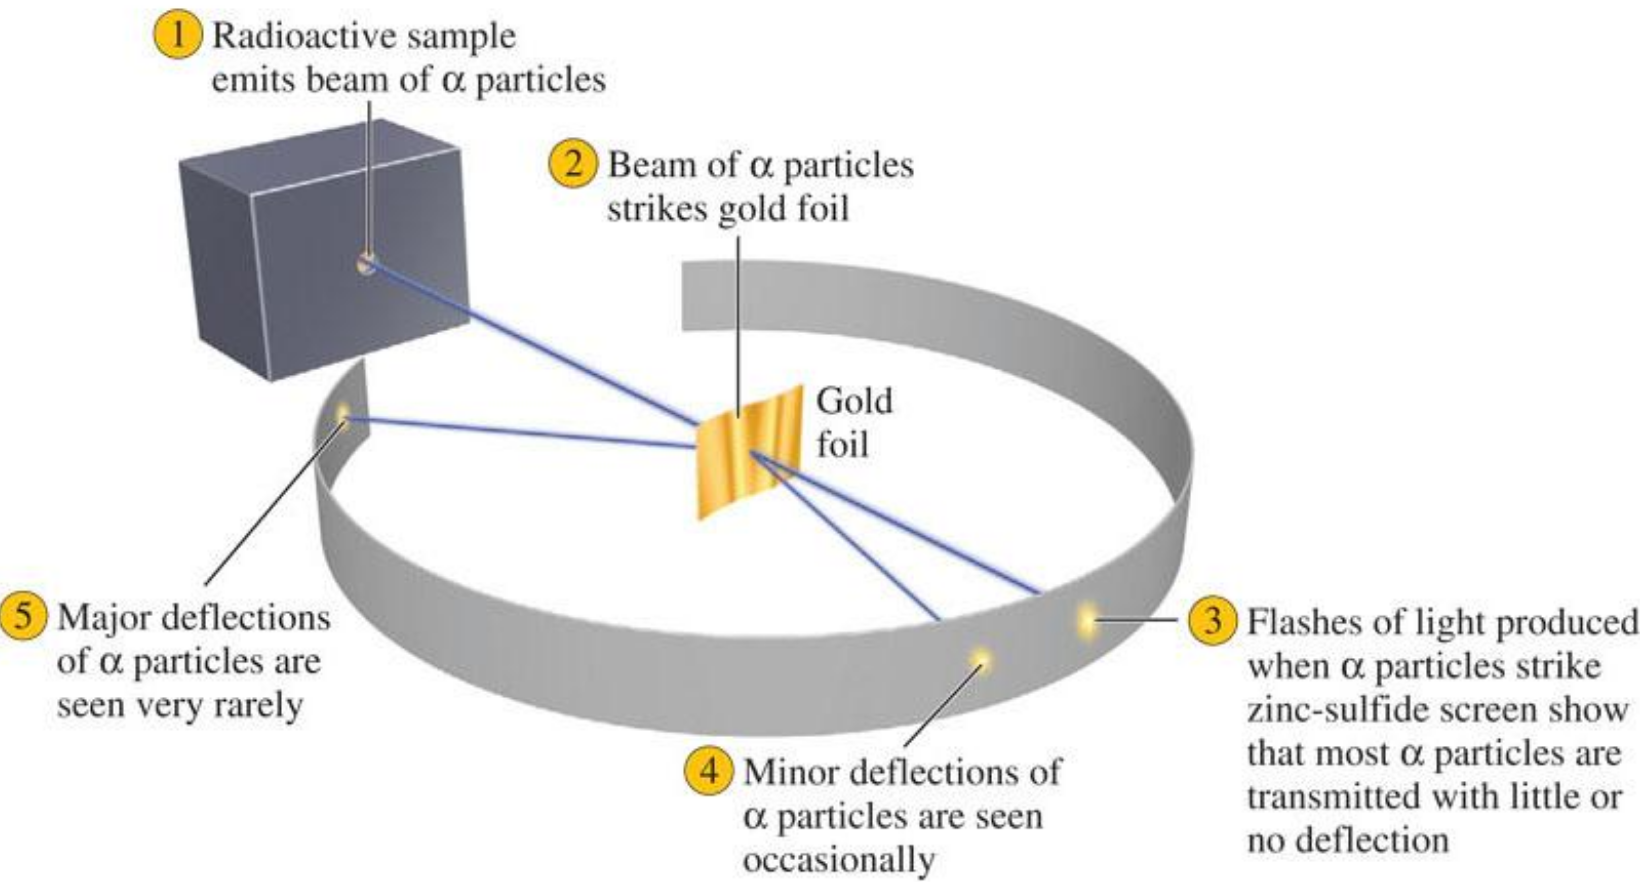
\includegraphics[scale=0.175]{alpha}
\end{frame}

\begin{frame}{Review: Modern Period Table}
  \centering
  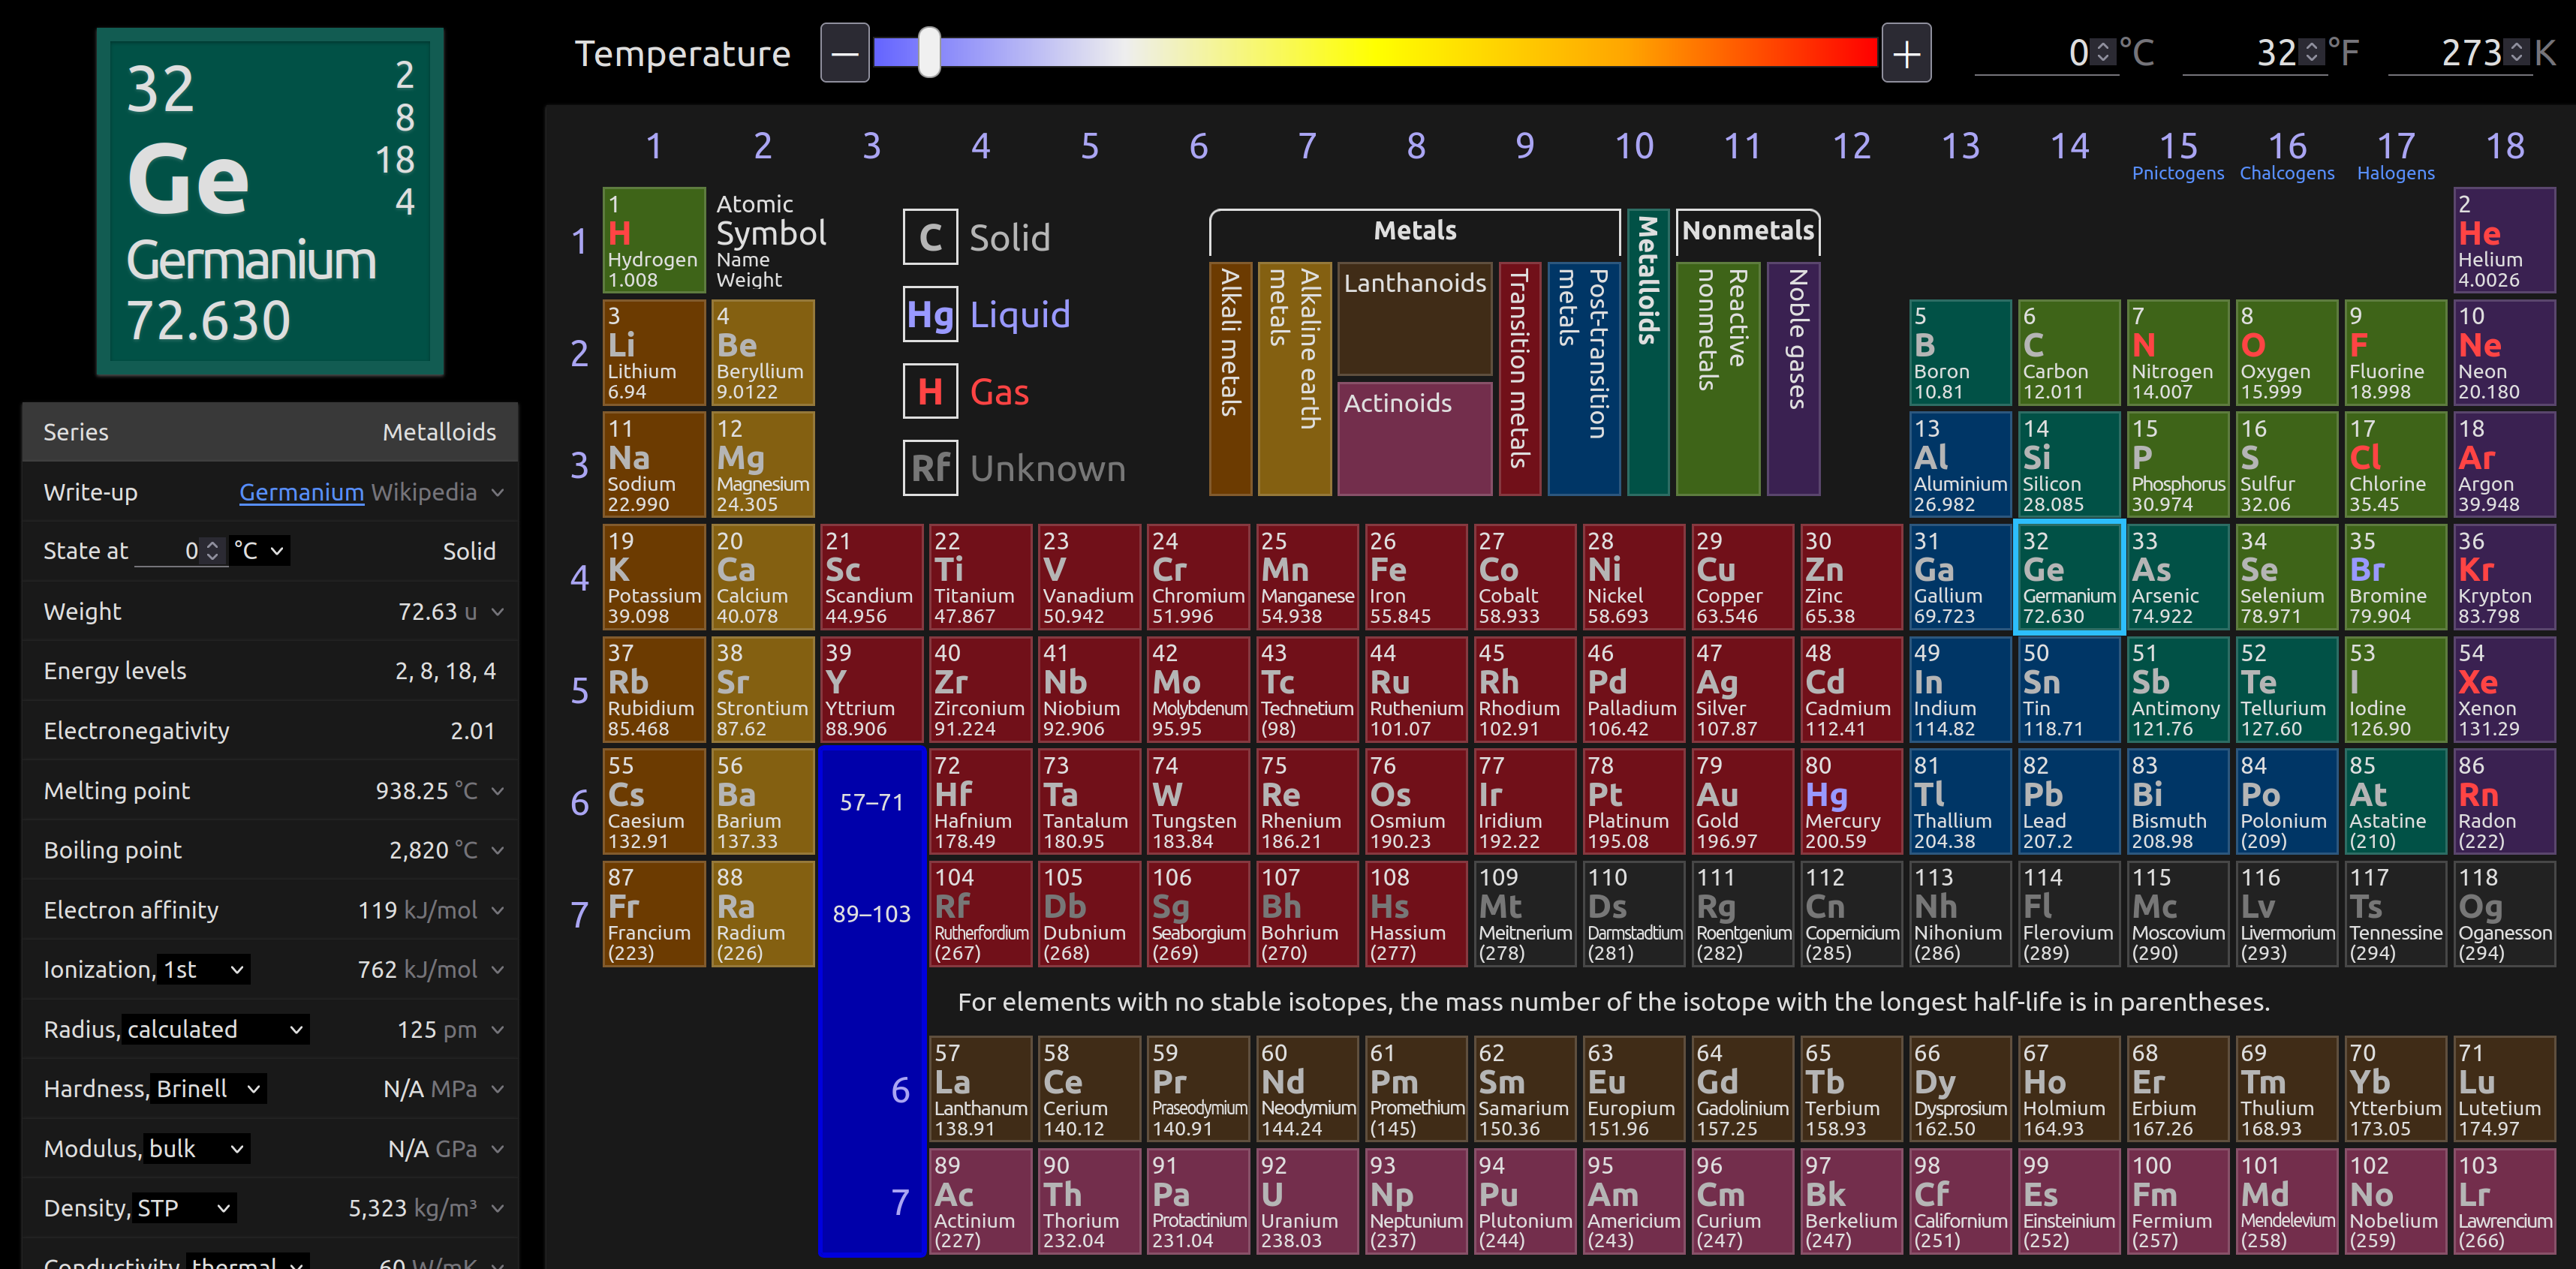
\includegraphics[width=\linewidth]{ptable}
\end{frame}

\begin{frame}{Relative Atomic Mass}
  \begin{equation}
    \text{Relative Atomic Mass} = (I_1\times A_1) + (I_2\times A_2) + \dots
  \end{equation}
  where $I$ is the mass of the isotope, and $A$ is the
  relative abundance between 0 and 1
\end{frame}

\begin{frame}{Defining Atomic Number and Mass}
  \begin{equation}
    ^\text{A}_\text{Z}\text{X}^\text{C}
  \end{equation}

  where A is the atomic mass, Z is the atomic number, X is atomic
  symbol, and C is the overall charge

  \textbf{Isotopes} - chemically same atom (same number of protons)
  but physically different (different number of neutrons)
\end{frame}

\begin{frame}{Hydrogen Isotopes and Applications}
  \begin{center}
    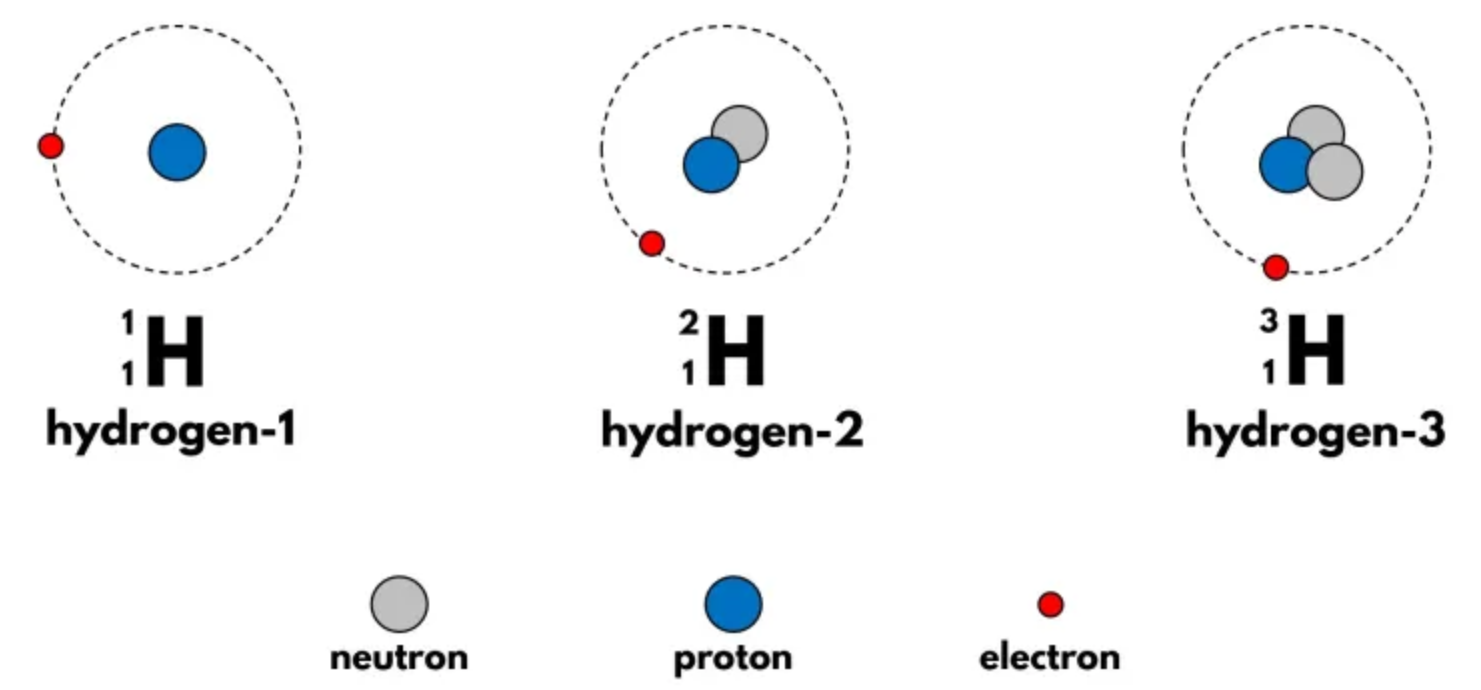
\includegraphics[width=0.75\linewidth]{hydro_iso}
  \end{center}

  \begin{itemize}
  \item Hydrogen ($^1_1$H), deuterium ($^2_1$D), and tritium ($^3_1$T)
    have relative abundances of $99.84\%$, $0.0156\%$, and trace amounts,
    respectively
  \item \textbf{Q:} Which hydrogen isostope is the highest in abundance?
  \end{itemize}
\end{frame}

\begin{frame}{Hydrogen Isostopes and Applications}
  \begin{center}
    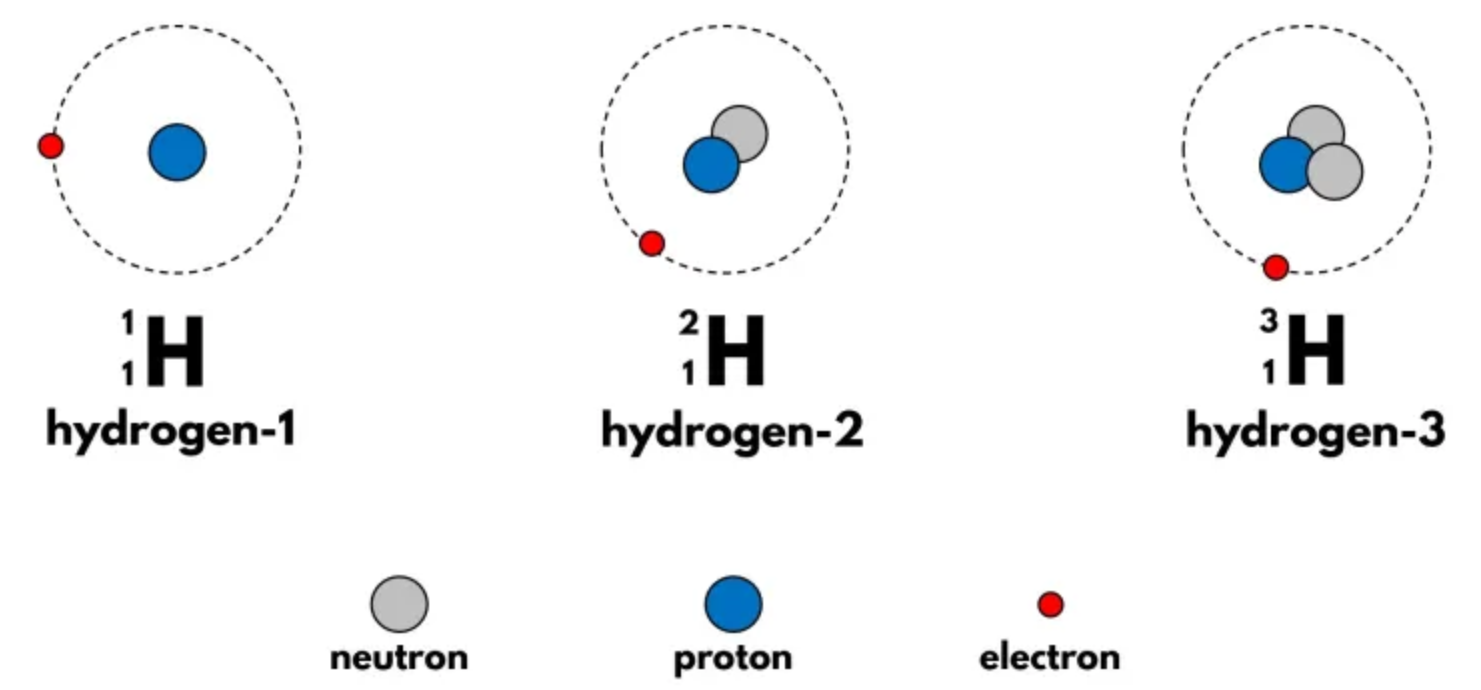
\includegraphics[width=0.75\linewidth]{hydro_iso}
  \end{center}

  \textbf{Applications}
  
  \begin{itemize}
  \item Semiconductor production enhancing Si-H bond by preventing
    chemical erosion and Hot Carrier Effect
  \item Chemical labeling to track chemical reactions
  \item Medicinal chemistry - FDA approved the first deuterium-labeled
    drug (\href{https://pubs.acs.org/doi/10.1021/acs.jmedchem.8b01808}{reference})
  \end{itemize}
\end{frame}

\begin{frame}{Experiment: Mass Spectroscopy}
  \begin{center}
    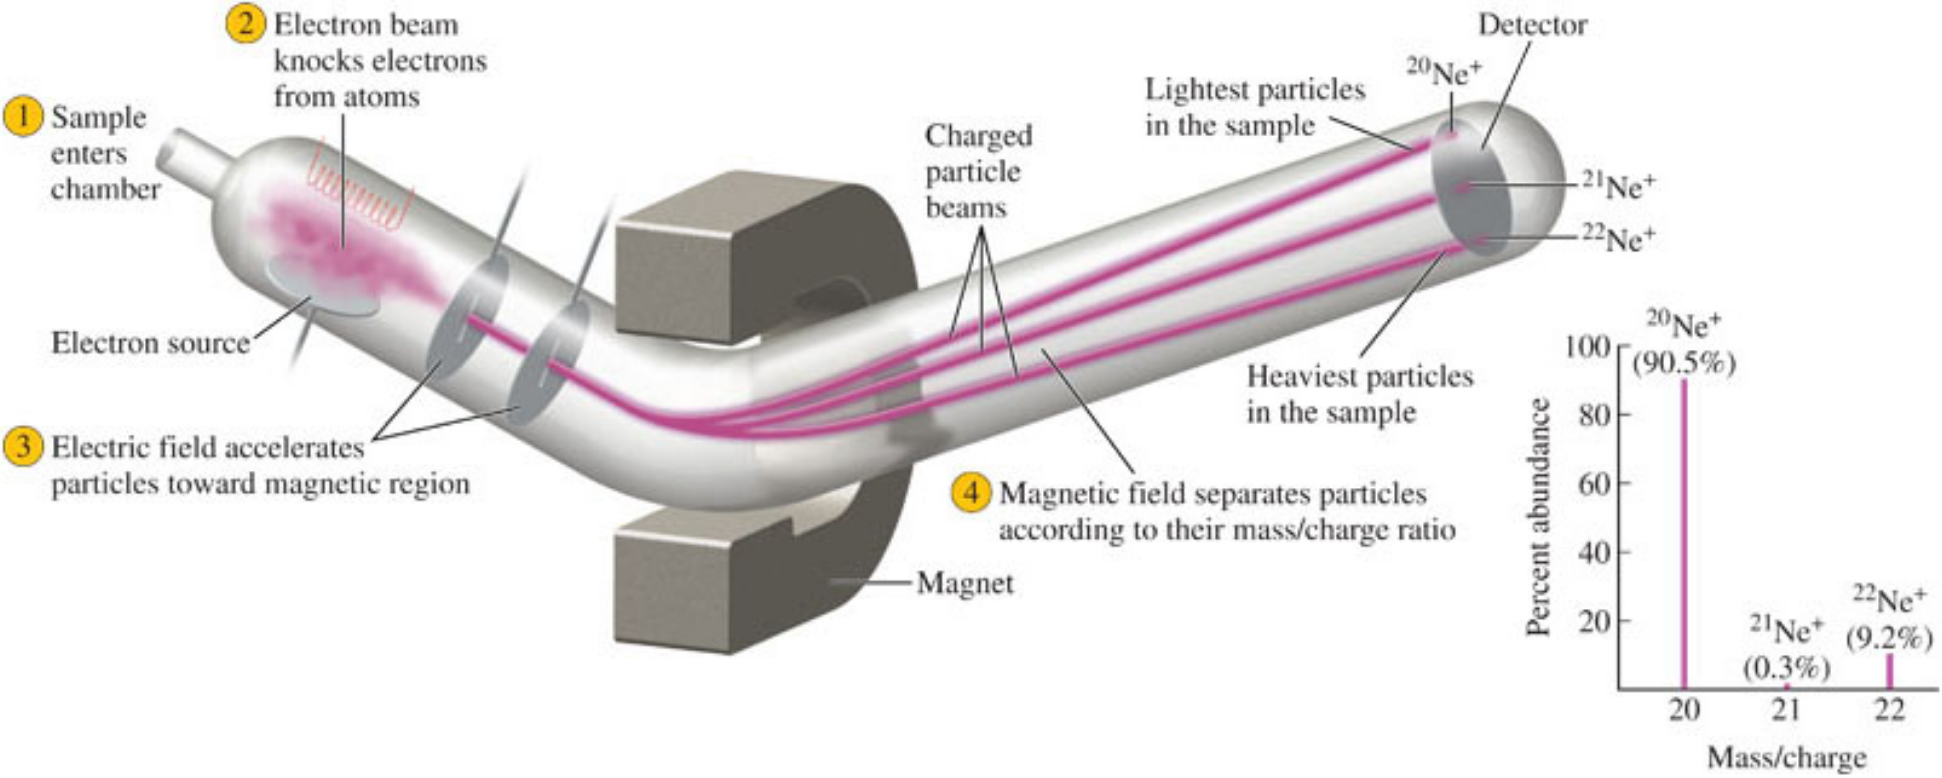
\includegraphics[width=\linewidth]{mass_spect}
  \end{center}

  \begin{itemize}
  \item Ionizes the atom and electric field accelerates atoms
  \item Time of flight - heavier atoms will travel slower
    than lighter ones
  \item Weighted average of atomic masses
  \end{itemize}  
\end{frame}

\section{Ionic and Molecular Compounds}

\begin{frame}{Ionic and Molecular Compounds}
  \textbf{Ionic Compounds}
  \begin{itemize}
  \item Consists of oppositely charged cations and anions
    such that the overall charge is neutral e.g CaCl$_2$(s),
    BaF(s), and Fe$_2$O$_3$(s)
  \item Electrolyte - substances that separate into the ions
    e.g. NaCl(aq) dissociates into Na$^+$ and Cl$^-$
  \item Forms ionic bonds (purely electrostatic interactions)
  \end{itemize}

  \textbf{Molecular Compounds}
  \begin{itemize}
  \item Composed of atoms from two or more nonmetals
  \item Forms covalent bonds (sharing of electrons)
  \end{itemize}
\end{frame}

\begin{frame}{Properties of Ionic and Molecular Compounds}
  \begin{center}
    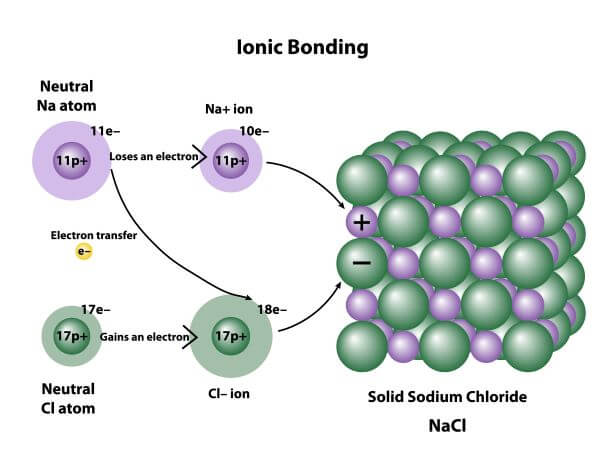
\includegraphics[width=0.6\linewidth]{Ionic-bond-example}
  \end{center}
  \vspace{-0.3in}
  \textbf{Ionic Compounds}
  \begin{itemize}
  \item Highly conductive and strong electrolyte - ability to
    carry electricity (electrons)
  \item High melting and boiling points, high density
  \end{itemize}
\end{frame}

\begin{frame}{Properties of Ionic and Molecular Compounds}
  \begin{center}
    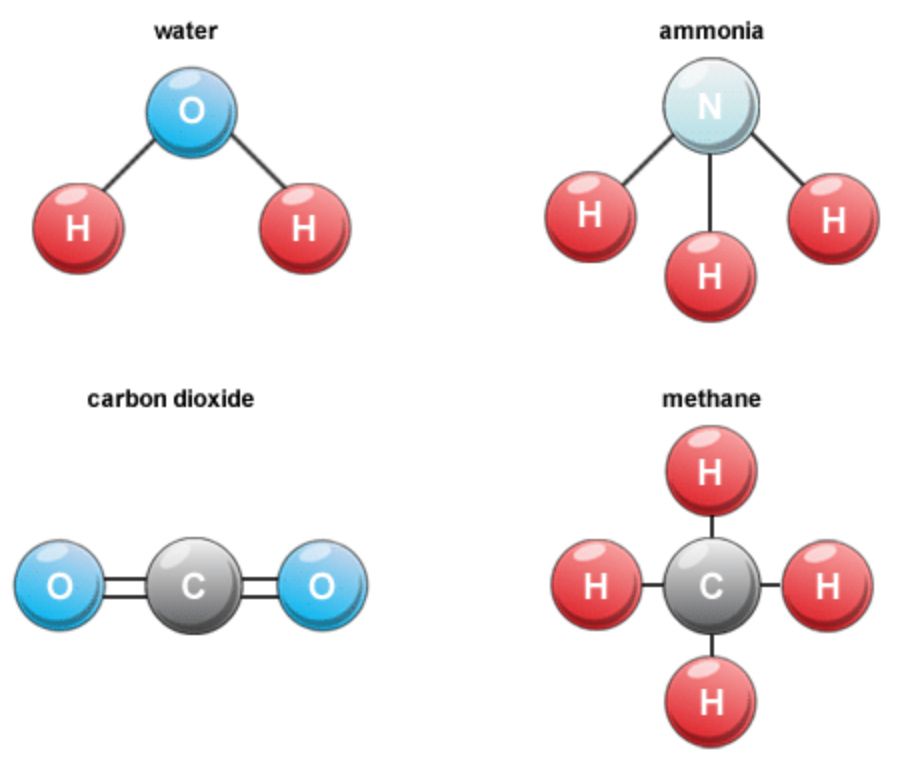
\includegraphics[width=0.6\linewidth]{molec_example}
  \end{center}
  \vspace{-0.3in}
  \textbf{Molecular Compounds}
  \begin{itemize}
  \item Not conductive and weak electrolyte
  \item Low melting and boiling points, low density
  \end{itemize}
\end{frame}


\begin{frame}{Introduction to Bonding}
  \textbf{Ionic Bonding}
  \begin{itemize}
  \item Electrons transferred from metal
    to nonmetal
  \item Ionized atoms and electrostatic interactions
  \end{itemize}

  \textbf{Covalent Bonding (CB)}
  \begin{itemize}
  \item Sharing of electrons between atoms (usually
    look at as pairs)
  \item Generally occurs between nonmetals in molecular
    elements, molecular compounds, and polyatomic ions
  \end{itemize}
\end{frame}

\begin{frame}{CB: Consideration of Electronegativity}
  \centering
  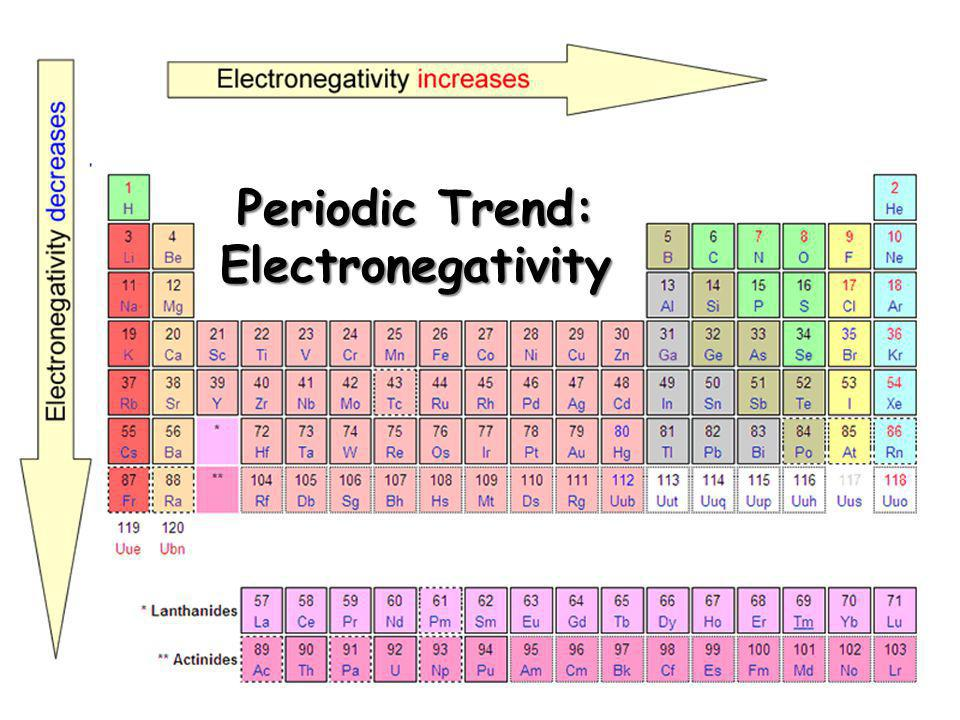
\includegraphics[width=\linewidth]{electronegativity}
\end{frame}

\begin{frame}{Pauling Electronegativity}
  Linus Pauling was the first one to describe electronegativity
  using bond energies. Determine the relative polarities of bonds
  or atoms tugging on the electrons

  \textbf{Examples:} Determine which atom does the electron
  gets pulled toward
  \begin{itemize}
  \item O-H
  \item C-H
  \item C-O
  \end{itemize}
\end{frame}

\begin{frame}{Practice: Bond Polarity within a Molecule}
  \begin{center}
    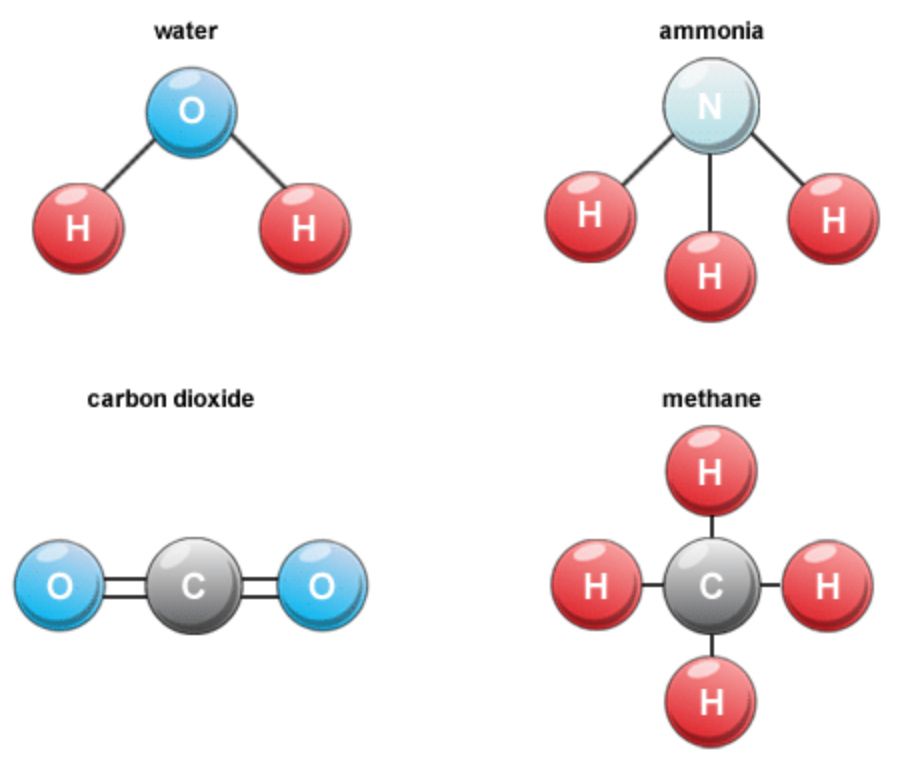
\includegraphics[width=0.6\linewidth]{molec_example}
  \end{center}
\end{frame}

\subsection{Monoatomic and Polyatomic Ions}

\begin{frame}{Monoatomic and Polyatomic Ions}
  \centering
  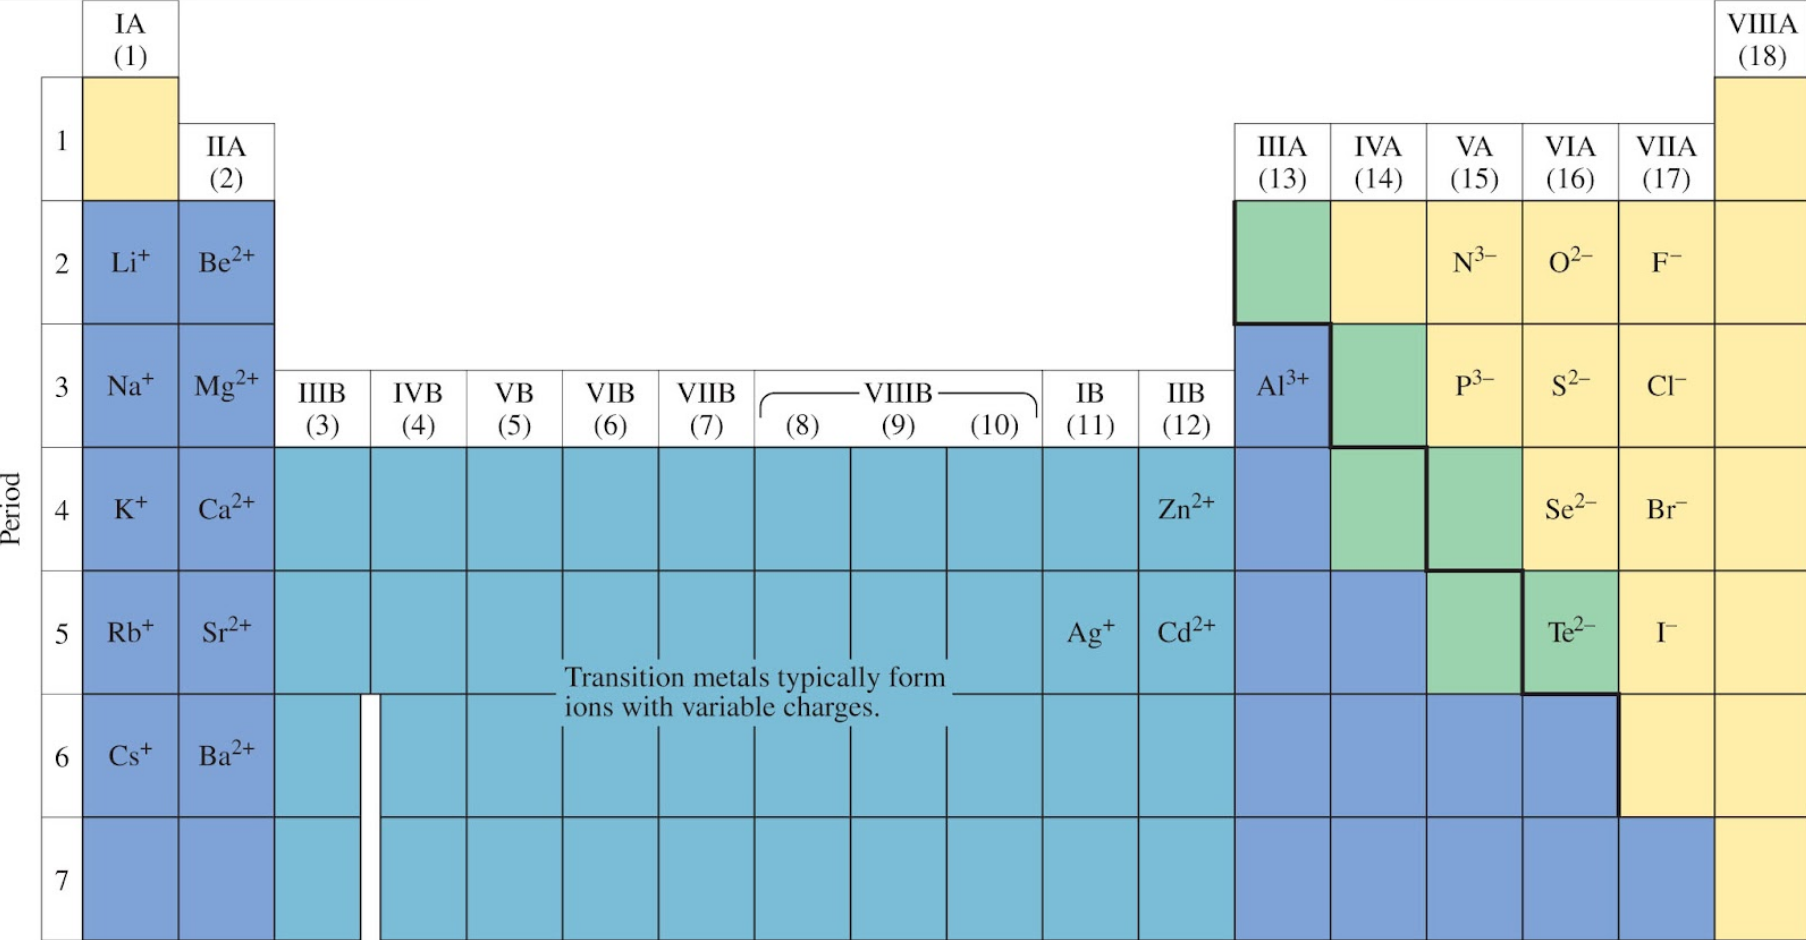
\includegraphics[width=\linewidth]{monoatomic_ion}
\end{frame}

\begin{frame}{Monoatomic and Polyatomic Ions}
  \centering
  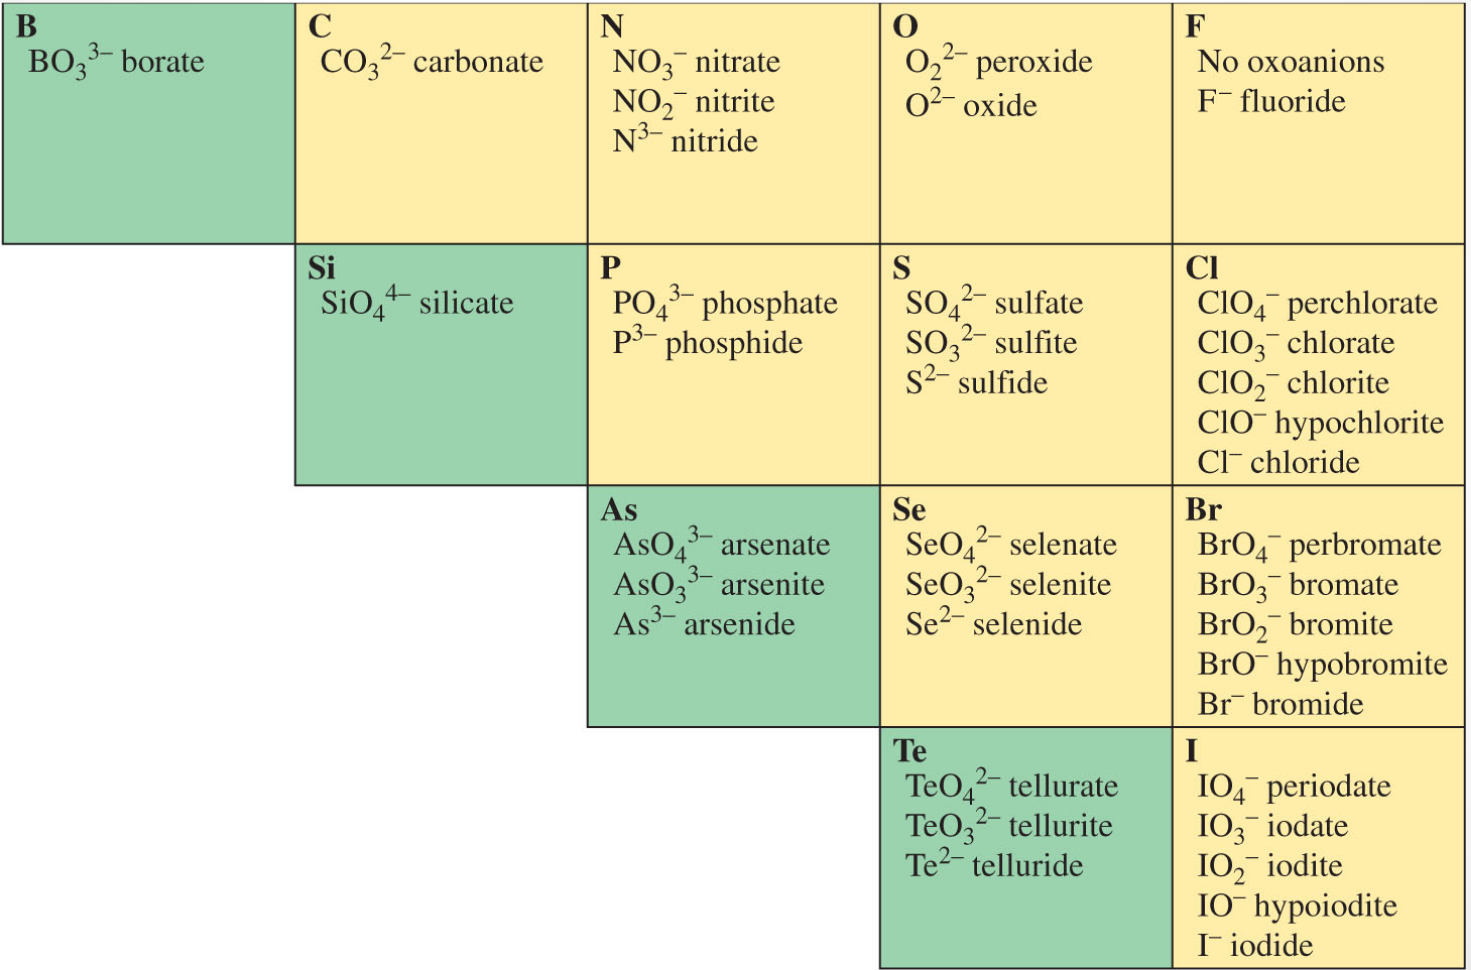
\includegraphics[width=\linewidth]{polyatomic_ion}
\end{frame}

\begin{frame}{Additional Polyatomic Ions}
  \centering
  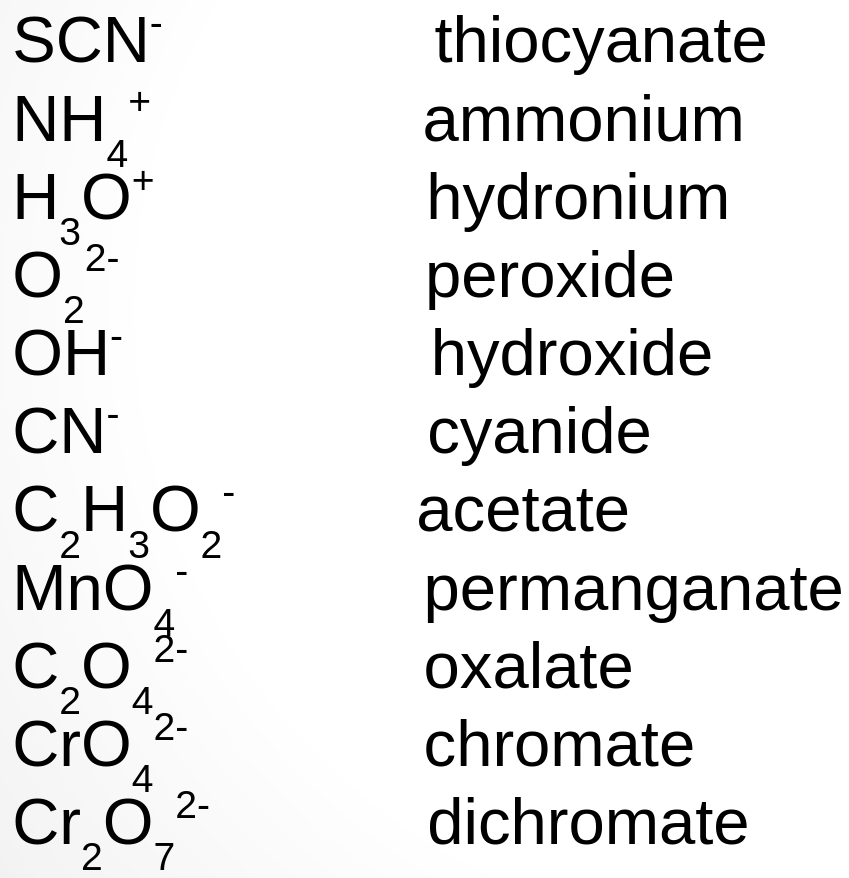
\includegraphics[width=0.7\linewidth]{more_poly_ions}
\end{frame}

\begin{frame}{Q: How is the overall charge determined?}
  This is based on the oxidation state of the atoms within
  the molecule. The total charge of the molecule is the sum of
  the atom oxidation state.
\end{frame}

\begin{frame}{Oxidation States Rules}
  \begin{enumerate}
  \item The oxidation state of an element is zero e.g  Xe, Cl$_2$, and S$_8$.
  \item The sum of the oxidation states of all the atoms or ions in a
    neutral compound is zero.
  \item The sum of the oxidation states of all the atoms in an ion is
    equal to the charge on the ion.
  \item The more electronegative element in a substance is assigned a
    negative oxidation state. The less electronegative element is assigned
    a positive oxidation state.
  \item Fluorine always has an oxidation state of -1
  \item Oxygen atoms normally have an oxidation state of -2
  \end{enumerate}
\end{frame}

\begin{frame}{Practice: Monoatomic and Polyatomic Ions}
  \centering
  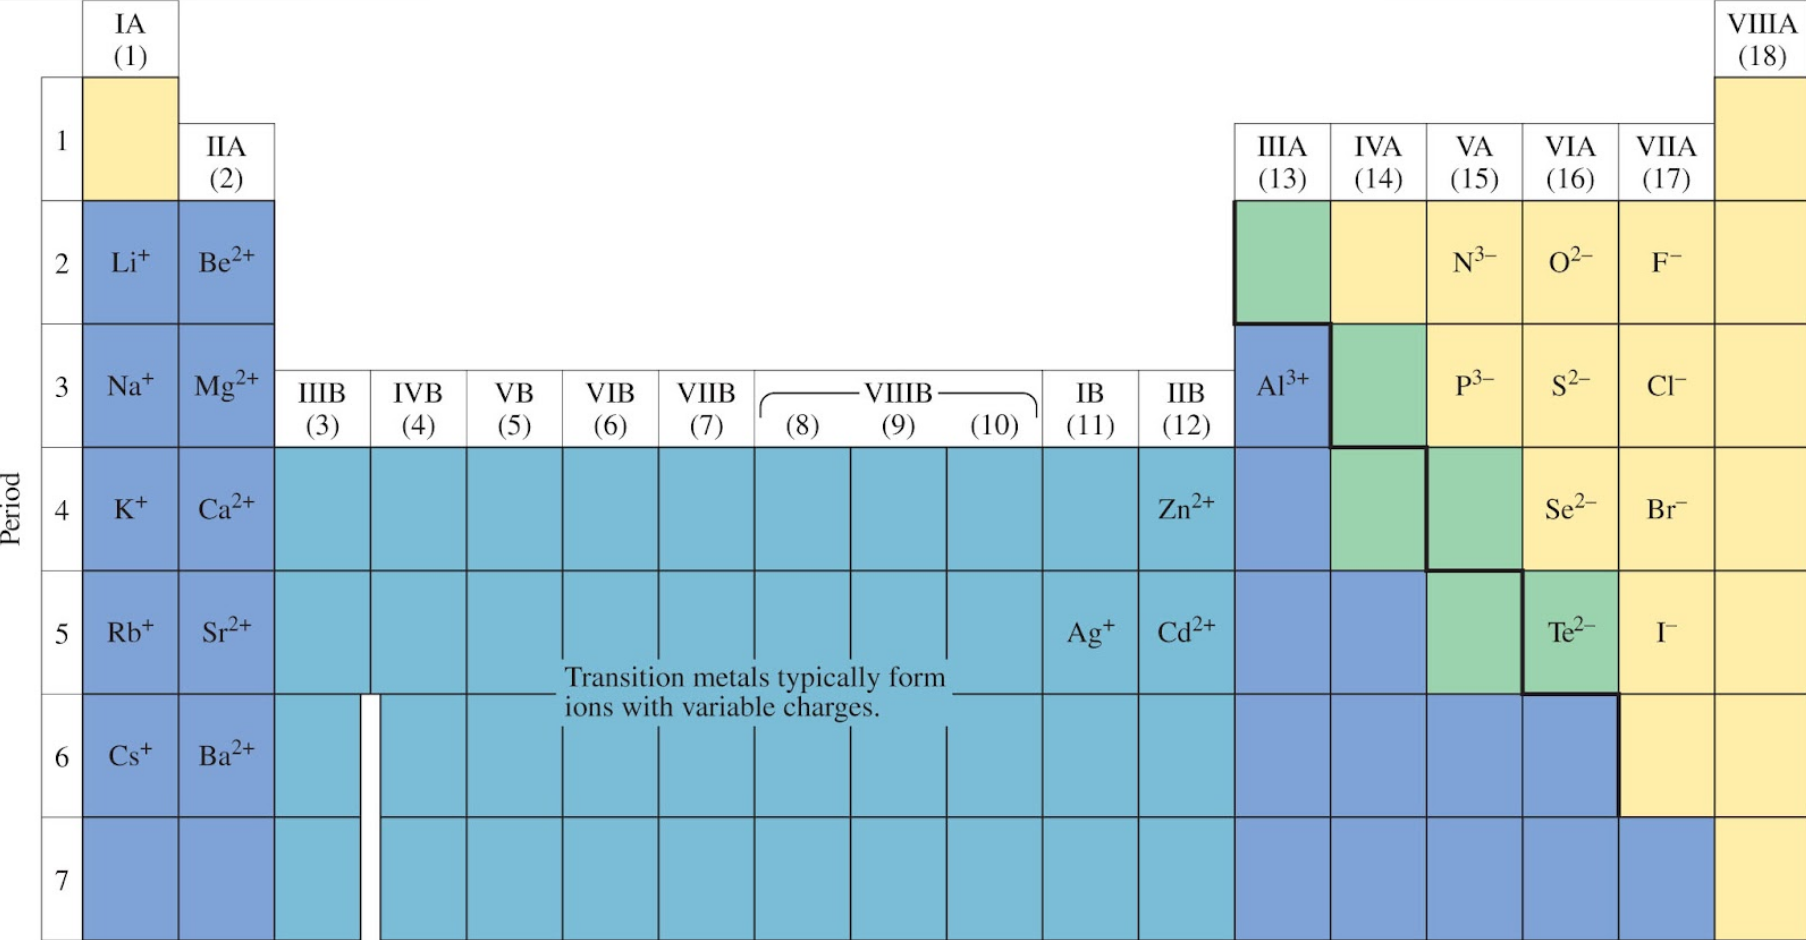
\includegraphics[width=\linewidth]{monoatomic_ion}
\end{frame}

\begin{frame}{Practice: Monoatomic and Polyatomic Ions}
  \centering
  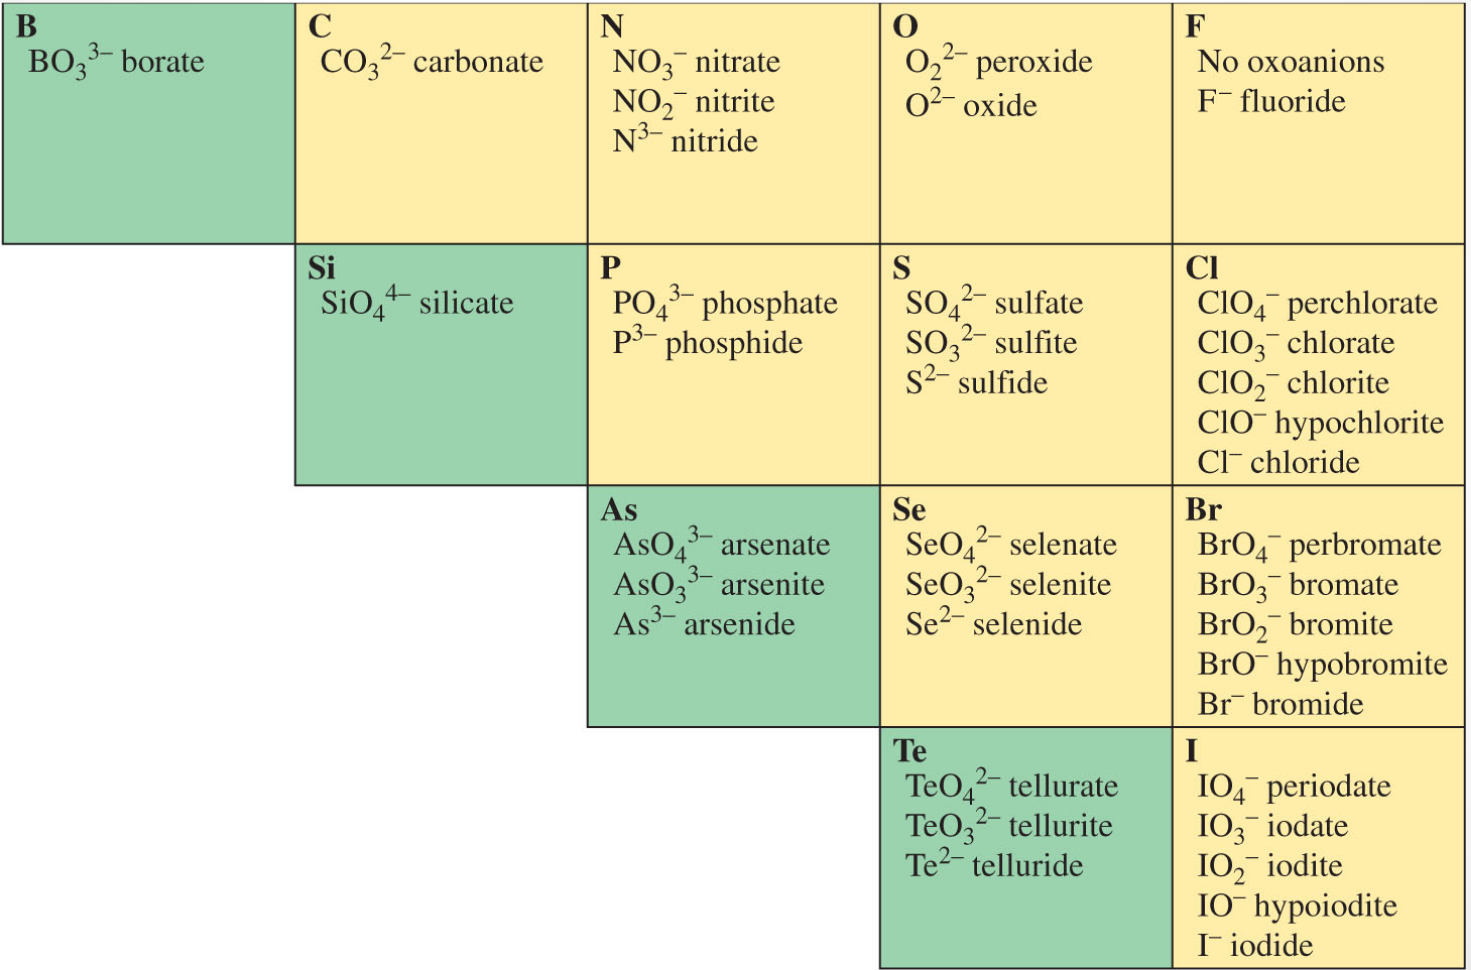
\includegraphics[width=\linewidth]{polyatomic_ion}
\end{frame}

\subsection{Formulas for Ionic Compounds}

\begin{frame}{Molecular Formulas for Ionic Compounds}
  The sum of the cations and anions equals to zero. The
  cation is written first then anion.

  \textbf{Examples:} Practice determining the oxidation states
  \begin{itemize}
  \item CaCO$_3$
  \item BaCl$_2$
  \item FeCl$_3$
  \item Ca(NO$_3$)$_2$
  \end{itemize}
\end{frame}

\section{Naming and Writing Formulas}

\subsection{Ionic Compounds}

\begin{frame}{Naming Ions}
  \textbf{Metals} - start with the element and end with ion

  \centering
  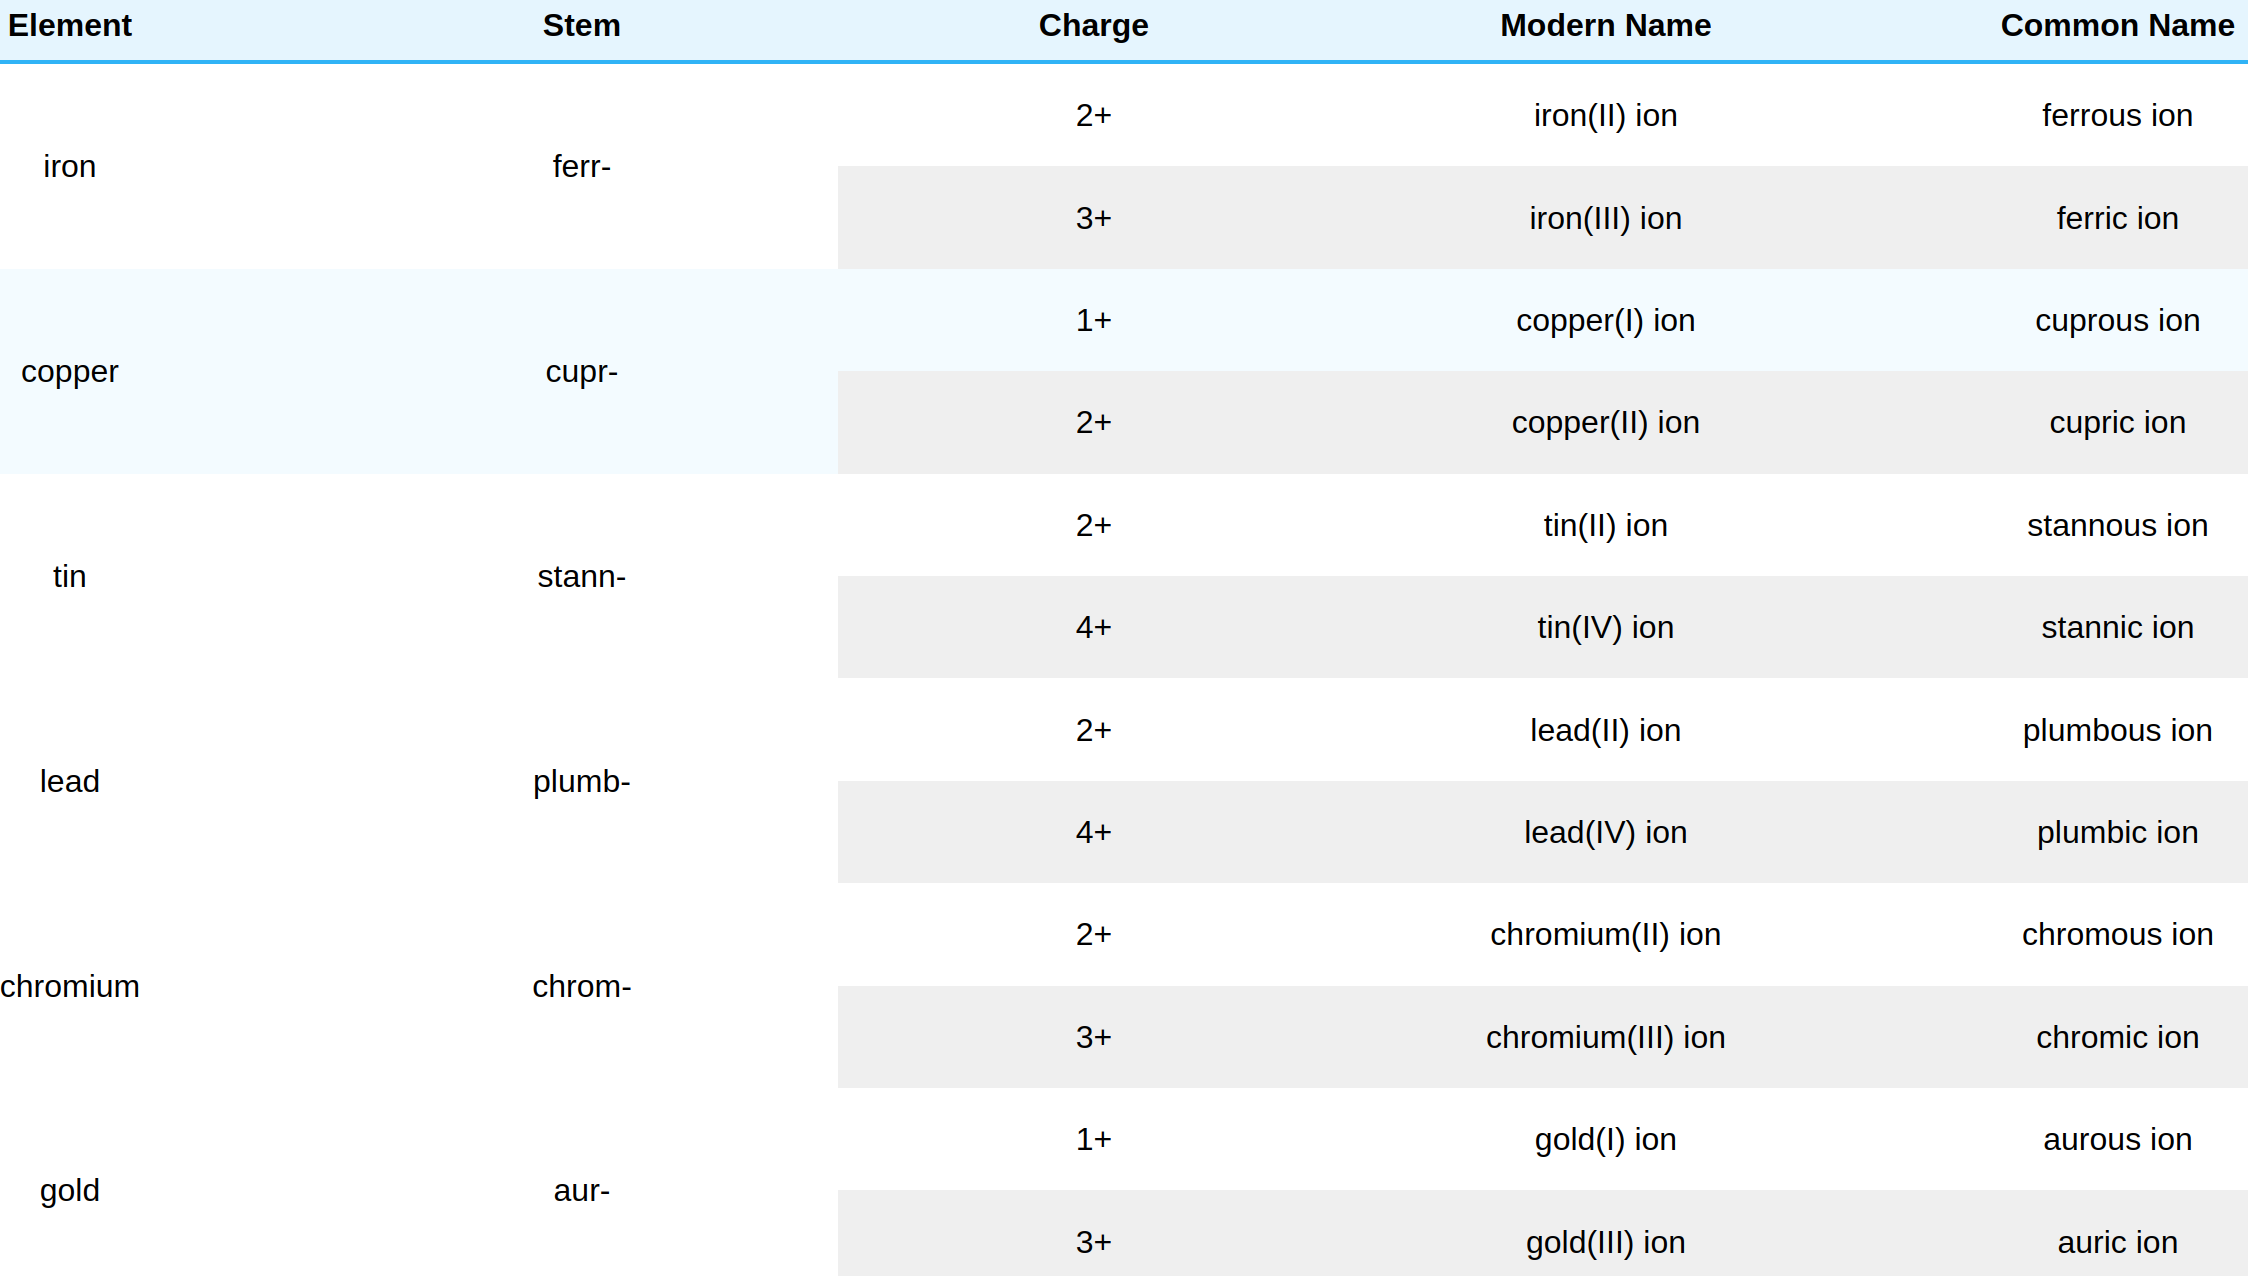
\includegraphics[width=\linewidth]{ions_names}
\end{frame}

\begin{frame}{Naming Nonmetal Ions}
  \textbf{Nonmetals} - replace suffix with -ide and end with ion

  \centering
  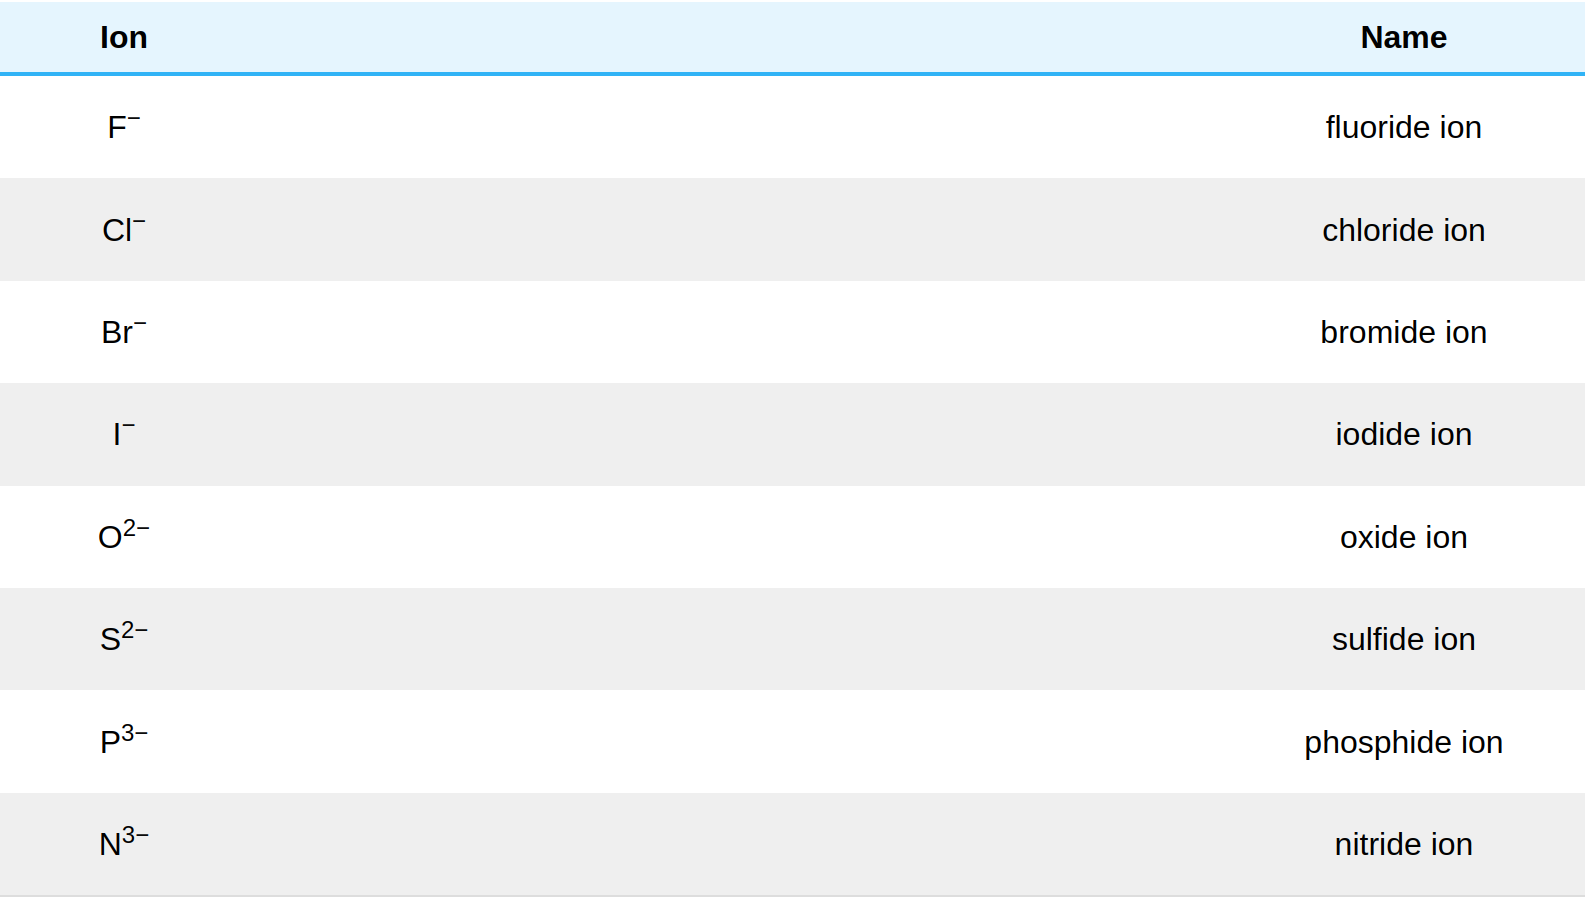
\includegraphics[width=\linewidth]{nonmetal_ions}
\end{frame}

\begin{frame}{Practice: Name Each Ion}
  \begin{itemize}
  \item Fe$^{2+}$
  \item F$^-$
  \item Ba$^+$
  \item S$^{2-}$
  \end{itemize}
\end{frame}

\begin{frame}{Naming Binary Ionic Compounds}
  The metal cation is named first, followed by the nonmetal anion.
  The word ion is dropped from both parts.

  \centering
  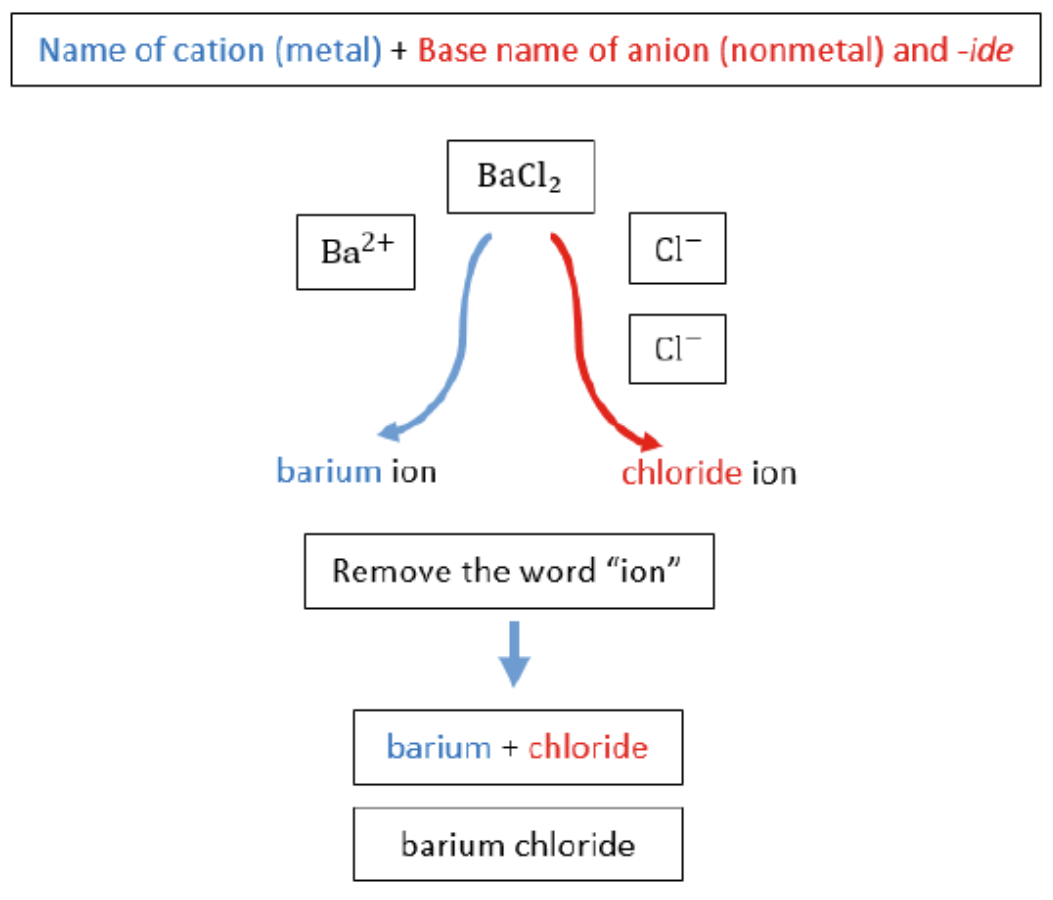
\includegraphics[width=0.7\linewidth]{barium_examp.png}
\end{frame}

\begin{frame}{Practice: Name the Ionic Compound}
  \begin{itemize}
  \item CaCl$_2$
  \item Ca$_3$P$_2$
  \item MgO
  \item FeCl$_2$
  \item Co$_2$O$_3$
  \end{itemize}
\end{frame}

\subsection{Molecular Compounds}

\begin{frame}{Naming Molecular Compounds}
  \begin{center}
    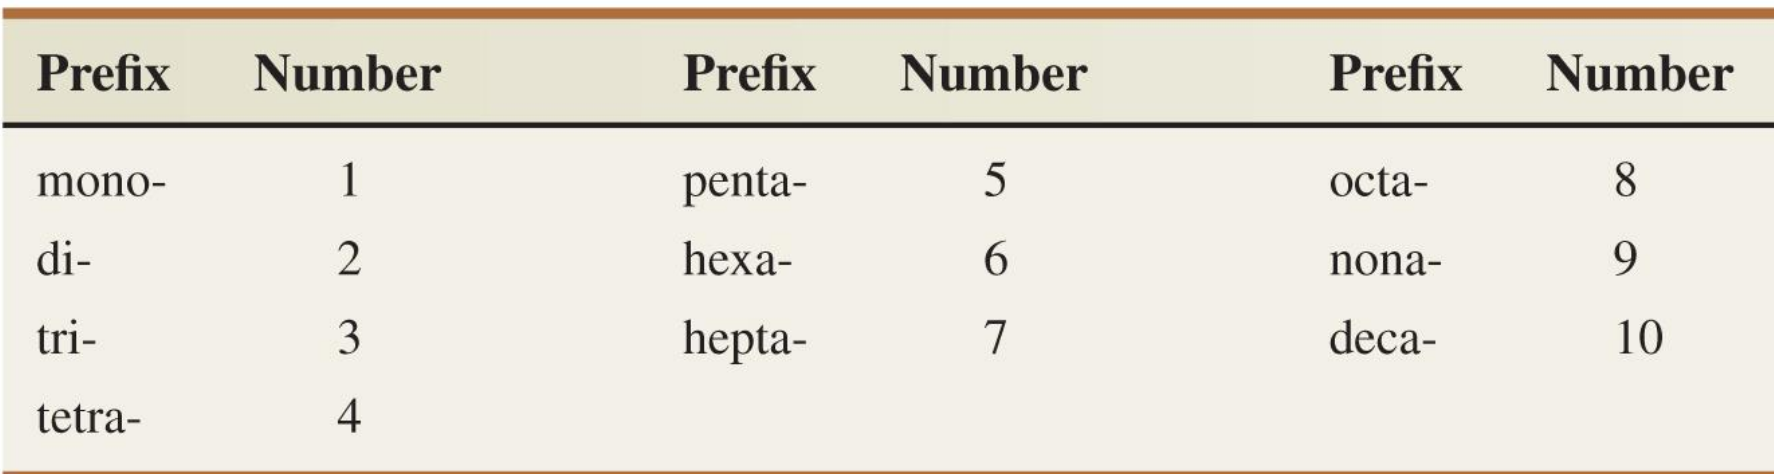
\includegraphics[width=\linewidth]{prefix_name}
  \end{center}
  
  \begin{enumerate}
  \item Use numerical prefix for the element (usually ignore the first
    when using ``mono'')
  \item Add ``-ide'' to the second element
  \end{enumerate}
\end{frame}

\begin{frame}{Naming Binary Molecular Compounds}
  \begin{itemize}
  \item H$_2$O
  \item N$_2$O$_4$
  \item CO
  \item CH$_4$
  \end{itemize}
\end{frame}

\subsection{Acids and Bases}

\begin{frame}{Naming Acids and Bases}
  \begin{center}
    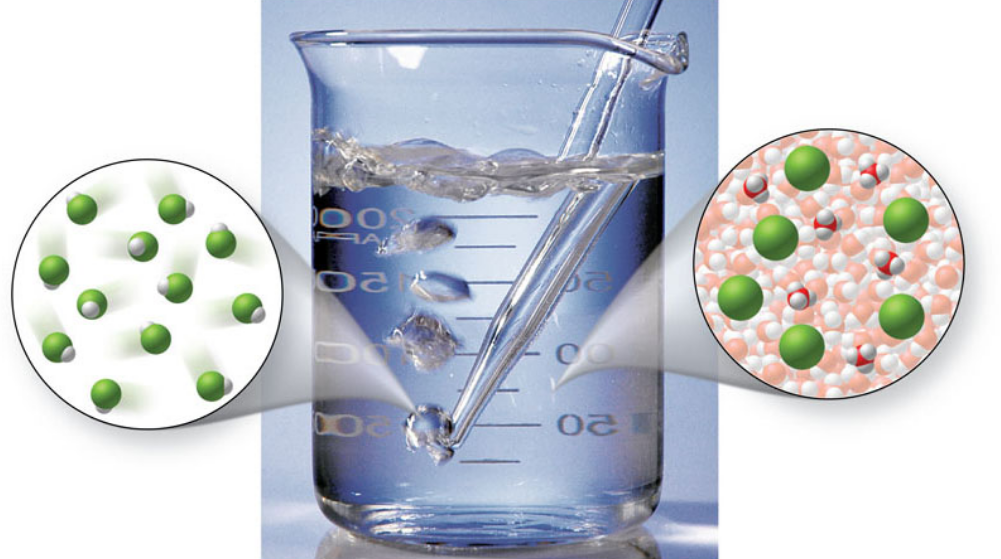
\includegraphics[width=0.5\linewidth]{acid_base}
  \end{center}

  \begin{enumerate}
  \item If anion ends in ``-ide,'' add ``hydro'' before the
    root of the anion name followed by ``-ic acid''
  \item If anion ends in ``-ate,'' use the root of the anion
    name followed by ``-ic acid''
  \item If anion ends in ``-ite,'' use the root of the anion
    name followed by ``-ous acid''
  \end{enumerate}
\end{frame}

\begin{frame}{Practice: Naming the Acid}
  \begin{itemize}
  \item HCl
  \item HNO$_3$
  \item H$_2$CO$_3$
  \item H$_2$SO$_3$
  \end{itemize}
\end{frame}

\begin{frame}{Definition(s) of an Acid}
  \textbf{Arrhenius Acid} - dissociation of acid in water to yield
  the ions e.g. HCl(aq) $\rightarrow$ H$^+$(aq) + Cl$^-$(aq)
  
  \textbf{Br{\o}nsted Acid} - any species that can donate a proton
  H$^+$

  \textbf{Lewis Acid} - donation of a pair of electrons
\end{frame}

\end{document}
